\section{Experimental Setup}
    The measurement equipment consists of the following elements: springs, Jolly balance, air track, electronic timer, electronic balance and masses.\\
    \begin{figure}[h]
        \centering
        \begin{minipage}{0.4\linewidth}
            A: Sliding bar with metric scale;\\
            H: Vernier for reading;\\
            C: Small mirror with a horizontal line in the middle;\\
            D: Fixed glass tube also with a horizontal line in the middle;\\
            G: Knob for ascending and descending the sliding bar;\\
            S: Spring attached to top of the bar A.\\
        \end{minipage}
        \hspace{0.8cm}
        \begin{minipage}{0.35\linewidth}
            \label{jolly}
            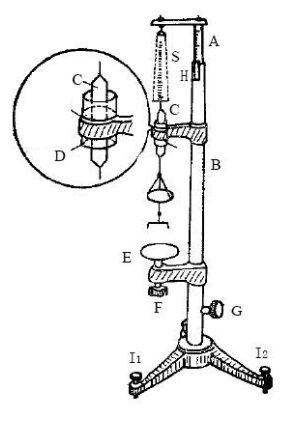
\includegraphics[height=6cm]{images/2.png}
        \end{minipage}
        \caption{Jolly balance}
    \end{figure}

    In order to measure the spring constant using the Jolly balance, we need to place the small mirror $C$ (see Figure \ref{jolly}) in the tube $D$ and make three lines coincide: the line on the mirror, the line on the glass tube and its reflection in the mirror. First, without adding any weight on the bottom end of the spring, adjust the knob G and make the three lines coincide. Then read the scale $L_1$.
    
    Second, add mass m to the bottom of the spring. The spring is stretched and the three lines no longer coincide. Adjust knob G to make them into one line again and read the corresponding number on scale $L_2$. The spring constant may be then found as
    \begin{equation}
        k=\frac{mg}{L_2-L_1}
    \end{equation}
    so that we can estimate the spring constant by finding a linear fit to the data using the least squares method.\\

    \begin{figure}[h]
        \centering
        \label{airtrack}
        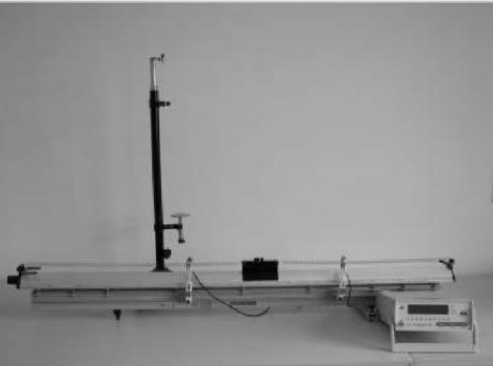
\includegraphics[height=6.5cm]{images/3.png}
        \caption{The experimental setup}
    \end{figure}

    A photoelectric measuring system consists of two photoelectric gates and an electronic timer. When a shutter on the object blocks the light, the computer will record the time. For period measurements, we use the I-shape shutter.

    When measuring the instaneous speed, the U-shape shutter is required. $\Delta t$ presents the time interval when the object travels a distance of $\Delta x=(x_{in}+x_{out})/2$. Hence we estimate the speed as $v=\Delta x/\Delta t$.

    \begin{figure}[h]
        \centering
        \label{U}
        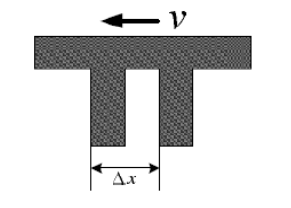
\includegraphics[height=3cm]{images/4.png}
        \caption{The U-shape shutter}
    \end{figure}